\section{Funções Compostas}

\begin{definition}
Sejam $f: X \to Y$ e $g: U \to V$ duas funções, com $Y \subset U$. A \textdef{função composta de $g$ com $f$} é a função denotada por $g \circ f$, com domínio em $X$ e contradomínio em $V$, que a cada elemento $x \in X$ faz corresponder o elemento $v = \prn{g \circ f}(x) = g(f(x)) \in V$. Diagramaticamente,
%
\begin{equation*}
\begin{array}{cccccc}
g \circ f : & X & \to     & Y \subset U & \to & V \\
     &  x & \mapsto & f(x) & \mapsto & g(f(x)).
\end{array}
\end{equation*}
\end{definition}

\begin{center}
     \tikzset{every picture/.style={line width=0.75pt}} %set default line width to 0.75pt        

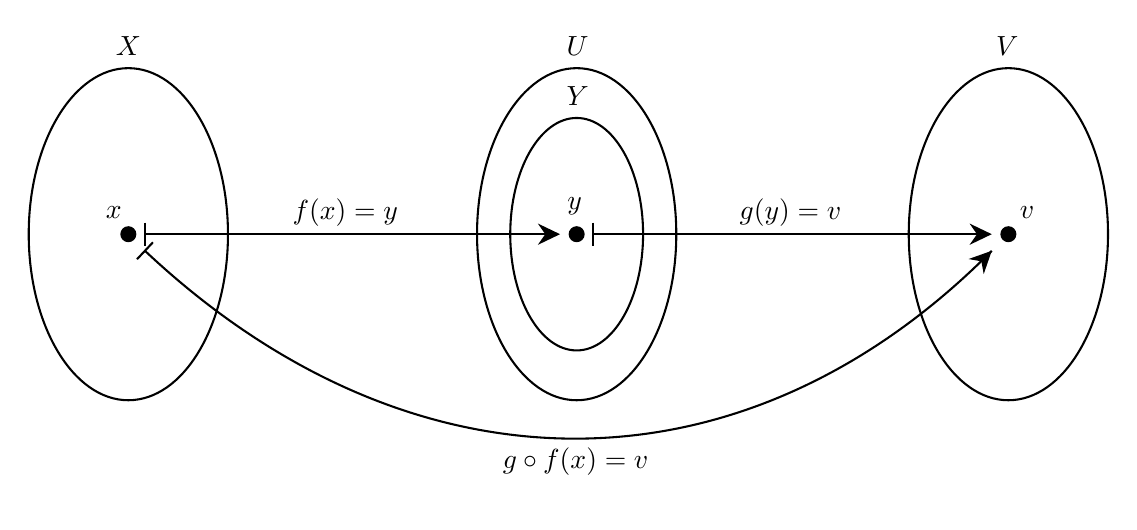
\begin{tikzpicture}[x=0.75pt,y=0.75pt,yscale=-1,xscale=1]
%uncomment if require: \path (0,308); %set diagram left start at 0, and has height of 308

%Shape: Ellipse [id:dp8584080168945698] 
\draw   (80,128) .. controls (80,83.82) and (101.49,48) .. (128,48) .. controls (154.51,48) and (176,83.82) .. (176,128) .. controls (176,172.18) and (154.51,208) .. (128,208) .. controls (101.49,208) and (80,172.18) .. (80,128) -- cycle ;
%Straight Lines [id:da9209150729175881] 
\draw    (128,128) ;

\draw [shift={(128,128)}, rotate = 0] [color={rgb, 255:red, 0; green, 0; blue, 0 }  ][fill={rgb, 255:red, 0; green, 0; blue, 0 }  ][line width=0.75]      (0, 0) circle [x radius= 3.35, y radius= 3.35]   ;
%Straight Lines [id:da7784202535308219] 
\draw    (552,128) ;

\draw [shift={(552,128)}, rotate = 0] [color={rgb, 255:red, 0; green, 0; blue, 0 }  ][fill={rgb, 255:red, 0; green, 0; blue, 0 }  ][line width=0.75]      (0, 0) circle [x radius= 3.35, y radius= 3.35]   ;
%Straight Lines [id:da4011502733578831] 
\draw    (136,128) -- (334,128) ;
\draw [shift={(336,128)}, rotate = 180] [fill={rgb, 255:red, 0; green, 0; blue, 0 }  ][line width=0.75]  [draw opacity=0] (10.72,-5.15) -- (0,0) -- (10.72,5.15) -- (7.12,0) -- cycle    ;
\draw [shift={(136,128)}, rotate = 180] [color={rgb, 255:red, 0; green, 0; blue, 0 }  ][line width=0.75]    (0,5.59) -- (0,-5.59)   ;
%Straight Lines [id:da7099724823991076] 
\draw    (344,128) ;

\draw [shift={(344,128)}, rotate = 0] [color={rgb, 255:red, 0; green, 0; blue, 0 }  ][fill={rgb, 255:red, 0; green, 0; blue, 0 }  ][line width=0.75]      (0, 0) circle [x radius= 3.35, y radius= 3.35]   ;
%Shape: Ellipse [id:dp6747907498340272] 
\draw   (296,128) .. controls (296,83.82) and (317.49,48) .. (344,48) .. controls (370.51,48) and (392,83.82) .. (392,128) .. controls (392,172.18) and (370.51,208) .. (344,208) .. controls (317.49,208) and (296,172.18) .. (296,128) -- cycle ;
%Shape: Ellipse [id:dp05220807095282054] 
\draw   (504,128) .. controls (504,83.82) and (525.49,48) .. (552,48) .. controls (578.51,48) and (600,83.82) .. (600,128) .. controls (600,172.18) and (578.51,208) .. (552,208) .. controls (525.49,208) and (504,172.18) .. (504,128) -- cycle ;
%Straight Lines [id:da13731439259167022] 
\draw    (352,128) -- (542,128) ;
\draw [shift={(544,128)}, rotate = 180] [fill={rgb, 255:red, 0; green, 0; blue, 0 }  ][line width=0.75]  [draw opacity=0] (10.72,-5.15) -- (0,0) -- (10.72,5.15) -- (7.12,0) -- cycle    ;
\draw [shift={(352,128)}, rotate = 180] [color={rgb, 255:red, 0; green, 0; blue, 0 }  ][line width=0.75]    (0,5.59) -- (0,-5.59)   ;
%Shape: Ellipse [id:dp3756659044594005] 
\draw   (312,128) .. controls (312,97.07) and (326.33,72) .. (344,72) .. controls (361.67,72) and (376,97.07) .. (376,128) .. controls (376,158.93) and (361.67,184) .. (344,184) .. controls (326.33,184) and (312,158.93) .. (312,128) -- cycle ;
%Curve Lines [id:da6306815692679878] 
\draw    (136,136) .. controls (264.33,256.67) and (424.33,256.67) .. (544,136) ;
\draw [shift={(544,136)}, rotate = 494.76] [fill={rgb, 255:red, 0; green, 0; blue, 0 }  ][line width=0.75]  [draw opacity=0] (10.72,-5.15) -- (0,0) -- (10.72,5.15) -- (7.12,0) -- cycle    ;
\draw [shift={(136,136)}, rotate = 223.24] [color={rgb, 255:red, 0; green, 0; blue, 0 }  ][line width=0.75]    (0,5.59) -- (0,-5.59)   ;

% Text Node
\draw (121,117.5) node   {$x$};
% Text Node
\draw (128,37.5) node   {$X$};
% Text Node
\draw (344.5,37.5) node   {$U$};
% Text Node
\draw (232.5,117.5) node   {$f(x) = y$};
% Text Node
\draw (447,117.5) node   {$g(y) = v$};
% Text Node
\draw (344.5,61.5) node   {$Y$};
% Text Node
\draw (551.5,37.5) node   {$V$};
% Text Node
\draw (343,114.5) node   {$y$};
% Text Node
\draw (561,117.5) node   {$v$};
% Text Node
\draw (343.5,237.5) node   {$g\circ f(x) = v$};

\end{tikzpicture}
\end{center}

\begin{example}
Seja $f: X \to Y$ uma função. Mostre que $f \circ \identity X = f$ e $\identity Y \circ f = f$.
\end{example}

\begin{solution}
Note que o domínio de $f \circ \identity X$ é $X$ já que $X$ é o domínio de $\identity X$. Logo, $f$ e $f \circ \identity X$ têm o mesmo domínio.
Um resultado análogo vale para o contradomínio dessas funções:  $Y$ também é contradomínio de $f \circ \identity X$ pois é o contradomínio de $f$.
Ademais, note que, para qualquer $x \in X$, 
%
\begin{align*}
(f \circ \identity X)\prn x &= f\prn{\identity X \prn x} \text{(definição de composição)} \\ &= f(x) \text{(definição de identidade)}.
\end{align*}
% 
Das igualdades de domínio, contradomínio e lei de associação de $f$ e $f \circ \identity X$, conclui-se que essas funções são iguais.

A demonstração da igualdade $\identity Y \circ f = f$ fica como exercício para o leitor.
\end{solution}

\begin{example}
\label{ex:comp-pq}
Dadas as funções $p$ e $q$ definidas no Exemplo \ref{example:func-sq-sqrt}, qual função resulta da composição $p \circ q$?
\end{example}

\begin{solution}
Pode-se representar a função $p \circ q$ com o seguinte diagrama:
%
\begin{equation*}
\begin{array}{cccccc}
p \circ q : & R_+ & \to     & \R \subset \R & \to     & \R_+ \\
            &  x  & \mapsto & \sqrt x       & \mapsto & \prn{\sqrt x}^2 = x.
\end{array}
\end{equation*}
%
Do diagrama, conclui-se que $p \circ q = \identity{\R_+}$.
\end{solution}

\begin{onlineact}[\khan{https://pt.khanacademy.org/math/algebra2/manipulating-functions/function-composition/e/compose-functions}{Encontre Funções Compostas}]
\end{onlineact}

\begin{onlineact}[\khan{https://pt.khanacademy.org/math/algebra2/manipulating-functions/combining-and-composing-modeling-functions/e/modeling-with-composite-functions}{Modele com Funções Compostas}]
\end{onlineact}